\documentclass{article}
\usepackage{amsmath}
\usepackage{hyperref}
\usepackage{url}
\usepackage{amssymb}
\usepackage{graphicx}
\usepackage{float}
\usepackage{bm}
\usepackage[top=2cm]{geometry}
\renewcommand{\thesubsubsection}{\thesubsection\ \alph{subsubsection})}

\title{Deep Learning - Homework 1}
\author{99222 - Frederico Silva, 99326 - Sebastião Carvalho}
\date{\today}

\begin{document}

\maketitle

\tableofcontents

\section{Question 1}

\subsection{Question 1.1}

\subsection{Question 1.2}

\subsection{Question 1.3}

\subsection{Question 1.4}

\section{Question 2}

\subsection{Question 2.1}

\subsection{Question 2.2}

\subsection{Question 2.3}

\section{Question 3}

\subsection{Question 3.1}
After running the code, the following plots were generated:

\begin{figure}[H]
    \centering
    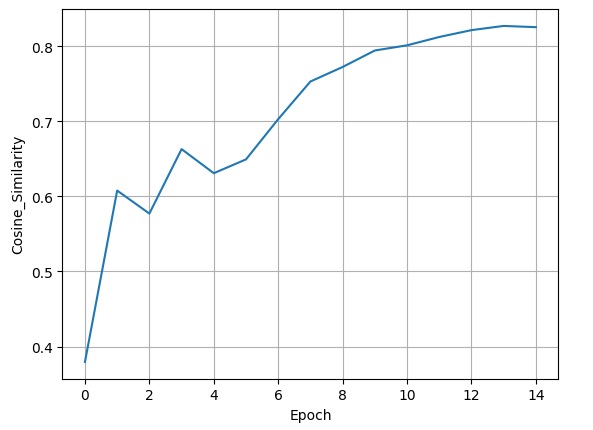
\includegraphics[width=0.8\textwidth]{../report/plots/RNN-cosine-similarity.png}
    \caption{Cosine similarity}
    \label{fig:cosine-similarity}
\end{figure}

\begin{figure}[H]
    \centering
    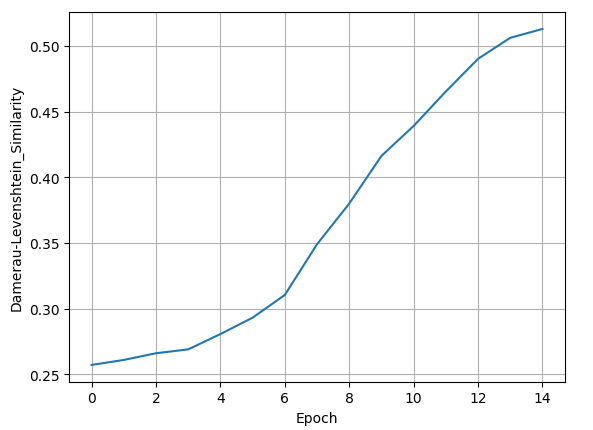
\includegraphics[width=0.8\textwidth]{../report/plots/RNN-dl-similarity.png}
    \caption{Damereau-Levenshtein similarity}
    \label{fig:dl-similarity}
\end{figure}

\begin{figure}[H]
    \centering
    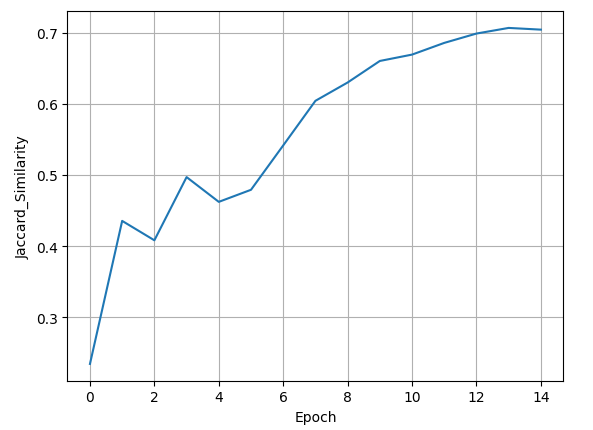
\includegraphics[width=0.8\textwidth]{../report/plots/RNN-jaccard-similarity.png}
    \caption{Jaccard similarity}
    \label{fig:jaccard-similarity}
\end{figure}

\begin{figure}[H]
    \centering
    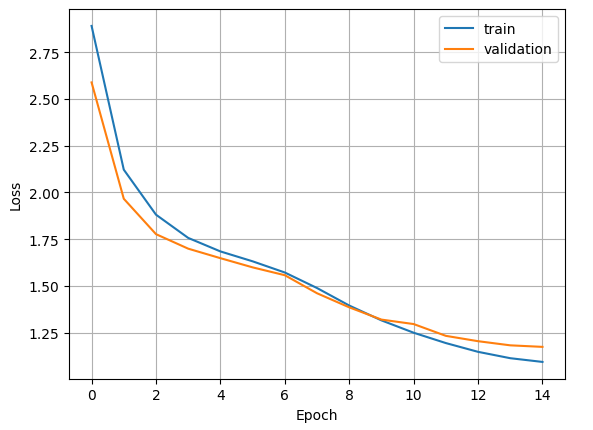
\includegraphics[width=0.8\textwidth]{../report/plots/RNN-valid-train-loss.png}
    \caption{Validation and training loss}
    \label{fig:valid-train-loss}
\end{figure}


In the test set, the jaccard similarity was 0.715, the cosine similarity was 0.832 and the damereau-levenshtein similarity was 0.509. The final test loss was 1.183.
\subsection{Question 3.2}

\subsection{Question 3.3}

\subsection{Question 3.4}

\section{Credits}

\section{Sources}

\end{document}